% !Mode:: "TeX:UTF-8"
% !TEX program = xelatex

%%%%%%%%%% Port for macOS %%%%%%%%%%%
% Modified: Qin Yubo

\def\usewhat{xelatex}
\documentclass[12pt,openany,twoside]{book}
%强制目录页的第一页的页眉页脚样式
\AtBeginDocument{\addtocontents{toc}{\protect\thispagestyle{only_foot}}}
                                                     % 本科生毕业论文通常采用单页排版
\input{setup/package}                                % 定义本文所使用宏包
\graphicspath{{figures/}}                            % 定义所有的图像文件在 figures 子目录下
\begin{document}                                     % 开始全文
% !Mode:: "TeX:UTF-8"
%  Authors: 张井   Jing Zhang: prayever@gmail.com     天津大学2010级管理与经济学部信息管理与信息系统专业硕士生
%           余蓝涛 Lantao Yu: lantaoyu1991@gmail.com  天津大学2008级精密仪器与光电子工程学院测控技术与仪器专业本科生

%%%%%%%%%% Fonts Definition and Basics %%%%%%%%%%%%%%%%%
\newcommand{\song}{\songti}    % 宋体
\newcommand{\fs}{\fangsong}        % 仿宋体
\newcommand{\kai}{\kaishu}      % 楷体
\newcommand{\hei}{\heiti}      % 黑体
\newcommand{\li}{\lishu}        % 隶书
\newcommand{\kaiGB}{\CJKfamily{kai}}      % 楷体GB2312, 用于独创性说明
\newcommand{\yihao}{\fontsize{26pt}{26pt}\selectfont}       % 一号, 1.倍行距
\newcommand{\xiaoyi}{\fontsize{24pt}{24pt}\selectfont}      % 小一, 1.倍行距
\newcommand{\erhao}{\fontsize{22pt}{1.25\baselineskip}\selectfont}       % 二号, 1.25倍行距
\newcommand{\xiaoer}{\fontsize{18pt}{18pt}\selectfont}      % 小二, 单倍行距
\newcommand{\sanhao}{\fontsize{16pt}{16pt}\selectfont}      % 三号, 1.倍行距
\newcommand{\xiaosan}{\fontsize{15pt}{15pt}\selectfont}     % 小三, 1.倍行距
\newcommand{\sihao}{\fontsize{14pt}{14pt}\selectfont}       % 四号, 1.0倍行距
\newcommand{\xiaosi}{\fontsize{12pt}{20pt}\selectfont}      % 小四, 1.倍行距
\newcommand{\wuhao}{\fontsize{10.5pt}{10.5pt}\selectfont}   % 五号, 单倍行距
\newcommand{\xiaowu}{\fontsize{9pt}{9pt}\selectfont}        % 小五, 单倍行距

\setmainfont{Times New Roman}

%\CJKcaption{gb_452}
%\CJKtilde  % 重新定义了波浪符~的意义
\newcommand\prechaptername{第}
\newcommand\postchaptername{章}

% 调整罗列环境的布局
\setitemize{leftmargin=3em,itemsep=0em,partopsep=0em,parsep=0em,topsep=-0em}
\setenumerate{leftmargin=3em,itemsep=0em,partopsep=0em,parsep=0em,topsep=0em}
%\setlength{\baselineskip}{20pt}
%\renewcommand{\baselinestretch}{1.38} % 设置行距

%避免宏包 hyperref 和 arydshln 不兼容带来的目录链接失效的问题。
\def\temp{\relax}
\let\temp\addcontentsline
\gdef\addcontentsline{\phantomsection\temp}

% 自定义项目列表标签及格式 \begin{publist} 列表项 \end{publist}
\newcounter{pubctr} %自定义新计数器
\newenvironment{publist}{%%%%%定义新环境
\begin{list}{[\arabic{pubctr}]} %%标签格式
    {
     \usecounter{pubctr}
     \setlength{\leftmargin}{2.5em}     % 左边界 \leftmargin =\itemindent + \labelwidth + \labelsep
     \setlength{\itemindent}{0em}     % 标号缩进量
     \setlength{\labelsep}{1em}       % 标号和列表项之间的距离,默认0.5em
     \setlength{\rightmargin}{0em}    % 右边界
     \setlength{\topsep}{0ex}         % 列表到上下文的垂直距离
     \setlength{\parsep}{0ex}         % 段落间距
     \setlength{\itemsep}{0ex}        % 标签间距
     \setlength{\listparindent}{0pt} % 段落缩进量
    }}
{\end{list}}%%%%%

\makeatletter
\renewcommand\normalsize{
  \@setfontsize\normalsize{12pt}{12pt} % 小四对应12pt
  \setlength\abovedisplayskip{4pt}
  \setlength\abovedisplayshortskip{4pt}
  \setlength\belowdisplayskip{\abovedisplayskip}
  \setlength\belowdisplayshortskip{\abovedisplayshortskip}
  \setlength{\baselineskip}{20pt} % 设置固定行间距为20pt
  \let\@listi\@listI}
\def\defaultfont{\renewcommand{\baselinestretch}{1.0}\normalsize\selectfont}
% 设置行距和段落间垂直距离
\renewcommand{\CJKglue}{\hskip -0.08pt plus 0.08\baselineskip} % 每行大概35个字符

\makeatother
%%%%%%%%%%%%% Contents %%%%%%%%%%%%%%%%% 目录样式修改,(天津大学关于博士、硕士学位论文统一格式的规定 2016.10.24)


\renewcommand{\contentsname}{目\qquad 录}
\setcounter{tocdepth}{2}
\titlecontents{chapter}[0em]{\vspace{0pt}\xiaosi\song}%
             {\prechaptername\thecontentslabel\postchaptername\quad}{} %
             {\hspace{.5em}\titlerule*[7pt]{.}\xiaosi\contentspage}
\titlecontents{section}[2em]{\vspace{0pt}\xiaosi\song} %
            {\thecontentslabel\quad}{} %
            {\hspace{.5em}\titlerule*[7pt]{.}\xiaosi\contentspage}
\titlecontents{subsection}[4em]{\vspace{0pt}\xiaosi\song} %
            {\thecontentslabel\quad}{} %
            {\hspace{.5em}\titlerule*[7pt]{.}\xiaosi\contentspage}
%\titlecontents{subsubsection}[6em]{\vspace{0pt}\xiaosi\song} %
%            {\thecontentslabel\quad}{} %
%            {\hspace{.5em}\titlerule*[7pt]{.}\xiaosi\contentspage}

%%%%%%%%%% Chapter and Section %%%%%%%%%%%%%%%%% 各级标题样式((天津大学关于博士、硕士学位论文统一格式的规定 2016.10.24))
\setcounter{secnumdepth}{4}
\setlength{\parindent}{2em}
\renewcommand{\chaptername}{\prechaptername\thechapter\postchaptername}
\titleformat{\chapter}{\centering\xiaosan\hei}{\chaptername}{1em}{}
\titlespacing{\chapter}{0pt}{33pt}{33pt}
\titleformat{\section}{\sihao\hei}{\thesection}{1em}{}
\titlespacing{\section}{0pt}{21pt}{21pt}
\titleformat{\subsection}{\sihao\hei}{\thesubsection}{1em}{}
\titlespacing{\subsection}{0pt}{13pt}{13pt}
\titleformat{\subsubsection}{\xiaosi\hei}{\thesubsubsection}{1em}{}
\titlespacing{\subsubsection}{0pt}{10pt}{10pt}

%%%%%%%%%% Table, Figure and Equation %%%%%%%%%%%%%%%%%
\renewcommand{\tablename}{表} % 插表题头
\renewcommand{\figurename}{图} % 插图题头
\renewcommand{\thefigure}{\arabic{chapter}-\arabic{figure}} % 使图编号为 7-1 的格式 %\protect{~}
\renewcommand{\thetable}{\arabic{chapter}-\arabic{table}}%使表编号为 7-1 的格式
\renewcommand{\theequation}{\arabic{chapter}-\arabic{equation}}%使公式编号为 7-1 的格式
\renewcommand{\thesubfigure}{(\alph{subfigure})}%使子图编号为 (a)的格式
\renewcommand{\thesubtable}{(\alph{subtable})} %使子表编号为 (a)的格式
\makeatletter
\renewcommand{\p@subfigure}{\thefigure~} %使子图引用为 7-1 a) 的格式,母图编号和子图编号之间用~加一个空格
\makeatother

\renewcommand{\arraystretch}{1.2}   % 扩大表格行距,以近似达到垂直居中
\setlength{\abovecaptionskip}{5pt}  % 图标标题文字与图或表之间的间隔
\setlength{\belowcaptionskip}{5pt}
%% 定制浮动图形和表格标题样式
\makeatletter
\long\def\@makecaption#1#2{%
   \vskip\abovecaptionskip
   \sbox\@tempboxa{\centering\wuhao\song{#1\qquad #2} }%
   \ifdim \wd\@tempboxa >\hsize
     \centering\wuhao\song{#1\qquad #2} \par
   \else
     \global \@minipagefalse
     \hb@xt@\hsize{\hfil\box\@tempboxa\hfil}%
   \fi
   \vskip\belowcaptionskip}
\makeatother
\captiondelim{~~~~} %用来控制longtable表头分隔符

%%%%%%%%%% Theorem Environment %%%%%%%%%%%%%%%%%
\theoremstyle{plain}
\theorembodyfont{\song\rmfamily}
\theoremheaderfont{\hei\rmfamily}
\newtheorem{theorem}{定理~}[chapter]
\newtheorem{lemma}{引理~}[chapter]
\newtheorem{axiom}{公理~}[chapter]
\newtheorem{proposition}{命题~}[chapter]
\newtheorem{corollary}{推论~}[chapter]
\newtheorem{definition}{定义~}[chapter]
\newtheorem{conjecture}{猜想~}[chapter]
\newtheorem{example}{例~}[chapter]
\newtheorem{remark}{注~}[chapter]
% \newtheorem{algorithm}{算法~}[chapter]
\newenvironment{proof}{\noindent{\hei 证明:}}{\hfill $ \square $ \vskip 4mm}
\theoremsymbol{$\square$}

%%%%%%%%%% Page: number, header and footer  %%%%%%%%%%%%%%%%%

%\frontmatter 或 \pagenumbering{roman}
%\mainmatter 或 \pagenumbering{arabic}
\makeatletter
\renewcommand\frontmatter{\clearpage
  \@mainmatterfalse
  \pagenumbering{Roman}} % 正文前罗马字体编号
\makeatother

%%%%%%%%%% References %%%%%%%%%%%%%%%%%
\renewcommand{\bibname}{参考文献}
% 重定义参考文献样式,来自thu
\makeatletter
\renewenvironment{thebibliography}[1]{%
   \chapter*{\bibname}%
   \xiaosi
   \list{\@biblabel{\@arabic\c@enumiv}}%
        {\renewcommand{\makelabel}[1]{##1\hfill}
         \setlength{\baselineskip}{17pt}
         \settowidth\labelwidth{0.5cm}
         \setlength{\labelsep}{0pt}
         \setlength{\itemindent}{0pt}
         \setlength{\leftmargin}{\labelwidth+\labelsep}
         \addtolength{\itemsep}{-0.7em}
         \usecounter{enumiv}%
         \let\p@enumiv\@empty
         \renewcommand\theenumiv{\@arabic\c@enumiv}}%
    \sloppy\frenchspacing
    \clubpenalty4000%
    \@clubpenalty \clubpenalty
    \widowpenalty4000%
    \interlinepenalty4000%
    \sfcode`\.\@m}
   {\def\@noitemerr
     {\@latex@warning{Empty `thebibliography' environment}}%
    \endlist\frenchspacing}
\makeatother

\addtolength{\bibsep}{3pt} % 增加参考文献间的垂直间距
\setlength{\bibhang}{2em} %每个条目自第二行起缩进的距离

% 参考文献引用作为上标出现
%\newcommand{\citeup}[1]{\textsuperscript{\cite{#1}}}
\makeatletter
    \def\@cite#1#2{\textsuperscript{[{#1\if@tempswa , #2\fi}]}}
\makeatother
%% 引用格式
\bibpunct{[}{]}{,}{s}{}{,}

%%%%%%%%%% Cover %%%%%%%%%%%%%%%%%
% 封面、摘要、版权、致谢格式定义
\makeatletter
\def\ctitle#1{\def\@ctitle{#1}}\def\@ctitle{}
\def\etitle#1{\def\@etitle{#1}}\def\@etitle{}
\def\caffil#1{\def\@caffil{#1}}\def\@caffil{}
\def\cmacrosubject#1{\def\@cmacrosubject{#1}}\def\@cmacrosubject{}
\def\cmacrosubjecttitle#1{\def\@cmacrosubjecttitle{#1}}\def\@cmacrosubjecttitle{}
\def\csubject#1{\def\@csubject{#1}}\def\@csubject{}
\def\csubjecttitle#1{\def\@csubjecttitle{#1}}\def\@csubjecttitle{}
\def\cgrade#1{\def\@cgrade{#1}}\def\@cgrade{}
\def\cauthor#1{\def\@cauthor{#1}}\def\@cauthor{}
\def\cauthortitle#1{\def\@cauthortitle{#1}}\def\@cauthortitle{}
\def\csupervisor#1{\def\@csupervisor{#1}}\def\@csupervisor{}
\def\csupervisortitle#1{\def\@csupervisortitle{#1}}\def\@csupervisortitle{}
\def\ccorsupervisor#1{\def\@ccorsupervisor{#1}}\def\@ccorsupervisor{}
\def\ccorsupervisortitle#1{\def\@ccorsupervisortitle{#1}}\def\@ccorsupervisortitle{}
\def\cfirstsubject#1{\def\@cfirstsubject{#1}}\def\@cfirstsubject{}   % “一级学科”
\def\cfirstsubjecttitle#1{\def\@cfirstsubjecttitle{#1}}\def\@cfirstsubjecttitle{} % 一级学科名称
\def\teachertable#1{\def\@teachertable{#1}}\def\@teachertable{}  % 答辩老师表格
\def\cdate#1{\def\@cdate{#1}}\def\@cdate{}
\def\declaretitle#1{\def\@declaretitle{#1}}\def\@declaretitle{}
\def\declarecontent#1{\def\@declarecontent{#1}}\def\@declarecontent{}
\def\authorizationtitle#1{\def\@authorizationtitle{#1}}\def\@authorizationtitle{}
\def\authorizationcontent#1{\def\@authorizationcontent{#1}}\def\@authorizationconent{}
\def\authorizationadd#1{\def\@authorizationadd{#1}}\def\@authorizationadd{}
\def\authorsigncap#1{\def\@authorsigncap{#1}}\def\@authorsigncap{}
\def\supervisorsigncap#1{\def\@supervisorsigncap{#1}}\def\@supervisorsigncap{}
\def\signdatecap#1{\def\@signdatecap{#1}}\def\@signdatecap{}
\long\def\cabstract#1{\long\def\@cabstract{#1}}\long\def\@cabstract{}
\long\def\eabstract#1{\long\def\@eabstract{#1}}\long\def\@eabstract{}
\def\ckeywords#1{\def\@ckeywords{#1}}\def\@ckeywords{}
\def\ekeywords#1{\def\@ekeywords{#1}}\def\@ekeywords{}

%在book文件类别下,\leftmark自动存录各章之章名,\rightmark记录节标题
\pagestyle{fancy}
%去掉章节标题中的数字 务必放到\pagestyle{fancy}之后才会起作用
%%不要注销这一行,否则页眉会变成:“第1章1  绪论”样式
\renewcommand{\chaptermark}[1]{\markboth{\chaptername~\ #1}{}}
  \fancyhf{}
%   \fancyhead[C]{\song\wuhao \leftmark} % 页眉显示章节名称
  \fancyhead[CO]{\song\wuhao \leftmark}  % 奇数页,显示章标题
  \fancyhead[CE]{\song\wuhao 天津大学硕士学位论文} % 偶数页,显示“天津大学硕士学位论文”
  \fancyfoot[C]{\song\xiaowu ~\thepage~}
  \renewcommand{\headrulewidth}{0.7pt}%
  \renewcommand{\footrulewidth}{0pt}%

\fancypagestyle{plain}{% 设置开章页页眉页脚风格
    \fancyhf{}%
    \fancyhead[C]{\song\wuhao \leftmark}
    \fancyfoot[C]{\song\xiaowu ~\thepage~ } %%首页页脚格式
    \renewcommand{\headrulewidth}{0.7pt}%
    \renewcommand{\footrulewidth}{0pt}%
}

\fancypagestyle{only_foot}{% 设置摘要、目录的页眉页脚风格:无页眉((天津大学关于博士、硕士学位论文统一格式的规定 2016.10.24)貌似要这种only_foot的样式)
    \fancyhf{}%
    \fancyfoot[C]{\song\xiaowu ~\thepage~ }
    \renewcommand{\headrulewidth}{0pt}%
    \renewcommand{\footrulewidth}{0pt}%
}


\newlength{\@title@width}
\def\@put@covertitle#1{\makebox[\@title@width][s]{#1}}
% 定义封面
\def\makecover{
\clearpage{\pagestyle{empty}\cleardoublepage}
   \phantomsection
    \pdfbookmark[-1]{\@ctitle}{ctitle}

    \begin{titlepage}
      \vspace*{0.8cm}
      \begin{center}

      \vspace*{1cm}
      \begin{center}
      \renewcommand{\baselinestretch}{1.25} % 设置行距
      \song\erhao\textbf{\@ctitle} % 修改成宋体加粗 (天津大学关于博士、硕士学位论文统一格式的规定, 2016.10.24)
      \renewcommand{\baselinestretch}{1.25} % 设置行距
      \end{center}
      \vspace*{1cm}

    %  \vspace*{1cm}

      \begin{center}
      \renewcommand{\baselinestretch}{1.25} % 设置行距
      \song\erhao\textbf{\@etitle}  % 修改成宋体加粗1.25倍行距(英文默认变成了Times new Roman) (天津大学关于博士、硕士学位论文统一格式的规定, 2016.10.24)
      \renewcommand{\baselinestretch}{1.25} % 设置行距
      \end{center}

      \vspace*{1cm} %3cm
      \setlength{\@title@width}{5em}
      {\song\sihao
      \begin{tabular}{p{\@title@width}@{:}l}
        \@put@covertitle{\@cfirstsubjecttitle} & \@cfirstsubject \\
        \@put@covertitle{\@csubjecttitle} & \@csubject \\
        \@put@covertitle{\@cauthortitle} & \@cauthor \\
        \@put@covertitle{\@csupervisortitle} & \@csupervisor \\
        \@put@covertitle{\@ccorsupervisortitle} & \@ccorsupervisor \\
      \end{tabular}
      }
      
      \vspace*{1cm}
      {\@teachertable}


  \vspace*{1.5cm}
  \song\sihao\@caffil \\
  \song\sihao\@cdate

\end{center}
%  另起一页: 独创性声明和学位论文版权使用授权书
\newpage
    \clearpage{\pagestyle{empty}\cleardoublepage} %去除空白页的页眉页脚(由于每章从奇数页开始因此有空白页)
    \thispagestyle{empty} %去掉页眉页脚
    \vspace*{1cm}
    \renewcommand{\baselinestretch}{1} % 设置行距
    \begin{center}\song\xiaoer{\@declaretitle}\end{center}\par
    \vspace*{0.5cm}
    \song\xiaosi{\@declarecontent}\par
    \vspace*{1cm}
    {\song\xiaosi
    \@authorsigncap \makebox[2.5cm][s]{}
    \@signdatecap \makebox[2cm][s]{} 年 \makebox[1cm][s]{} 月 \makebox[1cm][s]{} 日
    }

    \vspace*{3cm}
    \begin{center}\song\xiaoer{\@authorizationtitle}\end{center}\par
    \vspace*{1cm}
    {
    \song\xiaosi{\@authorizationcontent}

    \@authorizationadd\par
    }

    \vspace*{2cm}
    {\song\xiaosi\setlength{\parindent}{-0.45em}
    \begin{tabularx}{\textwidth}{ll}
        \@authorsigncap \makebox[3.5cm][s]{}  & \@supervisorsigncap \makebox[3.5cm][s]{}   \\
         &  \\
        \@signdatecap \makebox[1.5cm][s]{} 年 \makebox[1cm][s]{} 月 \makebox[1cm][s]{} 日 &
         \@signdatecap \makebox[1.5cm][s]{} 年 \makebox[1cm][s]{} 月 \makebox[1cm][s]{} 日 \\
    \end{tabularx}
    }
\end{titlepage}

%%%%%%%%%%%%%%%%%%%   Abstract and Keywords  %%%%%%%%%%%%%%%%%%%%%%%
\clearpage{\pagestyle{empty}\cleardoublepage} %去除空白页的页眉页脚(由于每章从奇数页开始因此有空白页)
\markboth{摘~要}{摘~要}
\addcontentsline{toc}{chapter}{摘\qquad 要}
\chapter*{\centering\song\erhao\textbf{摘\qquad 要}}
\thispagestyle{only_foot}

\setcounter{page}{1}
\song\defaultfont
\@cabstract
\vspace{\baselineskip}

%\hangafter=1\hangindent=52.3pt\noindent   %如果取消该行注释,关键词换行时将会自动缩进
\noindent
{\song\sihao\textbf{ 关键词:}} \@ckeywords

%%%%%%%%%%%%%%%%%%%   English Abstract  %%%%%%%%%%%%%%%%%%%%%%%%%%%%%%
\clearpage{\pagestyle{empty}\cleardoublepage} %去除空白页的页眉页脚(由于每章从奇数页开始因此有空白页)
\markboth{ABSTRACT}{ABSTRACT}
\addcontentsline{toc}{chapter}{ABSTRACT}
\chapter*{\centering\erhao\textbf{ABSTRACT}}
\thispagestyle{only_foot}
\@eabstract
\vspace{\baselineskip}

%\hangafter=1\hangindent=60pt\noindent  %如果取消该行注释,KEY WORDS换行时将会自动缩进
\noindent
{\sihao\textbf{KEY WORDS:}}  \@ekeywords
}

\makeatother                       % 完成对论文各个部分格式的设置
\frontmatter                               % 以下是论文导言部分,包括论文的封面,中英文摘要和中文目录
% % !Mode:: "TeX:UTF-8"

% %%  可通过增加或减少 setup/format.tex中的
% %%  第274行 \setlength{\@title@width}{8cm}中 8cm 这个参数来 控制封面中下划线的长度。

% \cheading{天津大学~2016~届本科生毕业论文}      % 设置正文的页眉,需要填上对应的毕业年份
% \ctitle{基于顾客有限理性预期的定价与供应链结构}    % 封面用论文标题,自己可手动断行
% \caffil{管理与经济学部} % 学院名称
% \csubject{工业工程}   % 专业名称
% \cgrade{2012~级}            % 年级
% \cauthor{秦昱博}            % 学生姓名
% \cnumber{3012209017}        % 学生学号
% \csupervisor{杨道箭}        % 导师姓名
% \crank{副教授}              % 导师职称

% \cdate{\the\year~年~\the\month~月~\the\day~日}

% \cabstract{
% 中文摘要一般在~400~字以内,简要介绍毕业论文的研究目的、方法、结果和结论,语言力求精炼。中英文摘要均要有关键词,一般为~3~—~7~个。字体为小四号宋体,各关键词之间要有分号。英文摘要应与中文摘要相对应,字体为小四号~Times New Roman,详见模板。
% }

% \ckeywords{关键词~1;关键词~2;关键词~3;……;关键词~7(关键词总共~3~—~7~个,最后一个关键词后面没有标点符号)}

% \eabstract{
% The upper bound of the number of Chinese characters is 400. The abstract aims at introducing the research purpose, research methods, research results, and research conclusion of graduation thesis, with refining words. Generally speaking, both the Chinese and English abstracts require the keywords, the number of which varies from 3 to 7, with a semicolon between adjacent words. The font of the English Abstract is Times New Roman, with the size of 12pt(small four).
% }

% \ekeywords{keyword 1, keyword 2, keyword 3, ……, keyword 7 (no punctuation at the end)}

% \makecover

% \clearpage


% !Mode:: "TeX:UTF-8"


\ctitle{基于生成式对抗网络的图像编辑与多模态图像转换}  %封面用论文标题,自己可手动断行
\etitle{Generative Adversarial Networks Based Image Editing and Multi Modal Image Translation}
\caffil{天津大学智能与计算学部} %学院名称
\cfirstsubjecttitle{\textbf{专业类别}}
\cfirstsubject{计算机技术}   %专业
\csubjecttitle{\textbf{研究方向}}
\csubject{计算机视觉}   %专业
\cauthortitle{\textbf{作者姓名}}     % 学位
\cauthor{刘家旭}   %学生姓名
\csupervisortitle{\textbf{指导教师}}
\csupervisor{朱鹏飞~~副教授} %导师姓名
\ccorsupervisortitle{\textbf{企业导师}}
\ccorsupervisor{刘昕} %导师姓名

\teachertable{
\begin{table}[h]
\centering
\song\xiaosi{
\begin{tabularx}{\textwidth}{|*{4}{>{\centering\arraybackslash}X|}}
\hline
\textbf{答辩日期}                & \multicolumn{3}{c|}{2021 年   月   日}       \\ \hline
\textbf{答辩委员会}               & \textbf{姓名} & \textbf{职称} & \textbf{工作单位} \\ \hline
\textbf{主席}                  &             &             &               \\ \hline
\multirow{2}{*}{\textbf{委员}} &             &             &               \\ \cline{2-4} 
                             &             &             &               \\ \hline
\end{tabularx}}
\end{table}}


\declaretitle{独创性声明}
\declarecontent{
本人声明所呈交的学位论文是本人在导师指导下进行的研究工作和取得的研究成果,除了文中特别加以标注和致谢之处外,论文中不包含其他人已经发表或撰写过的研究成果,也不包含为获得 {\underline{\kaiGB{\sihao{\textbf{~~天津大学~~}}}}} 或其他教育机构的学位或证书而使用过的材料。与我一同工作的同志对本研究所做的任何贡献均已在论文中作了明确的说明并表示了谢意。
}
\authorizationtitle{学位论文版权使用授权书}
\authorizationcontent{
本学位论文作者完全了解{\underline{\kaiGB{\sihao{\textbf{~~天津大学~~}}}}}有关保留、使用学位论文的规定。特授权{\underline{\kaiGB{\sihao{\textbf{~~天津大学~~}}}}} 可以将学位论文的全部或部分内容编入有关数据库进行检索,并采用影印、缩印或扫描等复制手段保存、汇编以供查阅和借阅。同意学校向国家有关部门或机构送交论文的复印件和磁盘。
}
\authorizationadd{(保密的学位论文在解密后适用本授权说明)}
\authorsigncap{学位论文作者签名:}
\supervisorsigncap{导师签名:}
\signdatecap{签字日期:}


\cdate{\CJKdigits{\the\year} 年\CJKnumber{\the\month} 月 \CJKnumber{\the\day} 日}
% 如需改成二零一二年四月二十五日的格式,可以直接输入,即如下所示
\cdate{二零二一年十月}
% \cdate{\the\year 年\the\month 月 \the\day 日} % 此日期显示格式为阿拉伯数字 如2012年4月25日
\cabstract{

生成式对抗网络(Generative Adversarial Nets,GANs)是2014年由Goodfellow等人提出的基于对抗训练的生成模型,伴随着深度学习的发展,GANs采用了更加高效的网络结构,同时研究人员不断提出更适合对抗训练的损失函数,GANs生成数据的质量有了很大提高,目前已广泛用于图像生成、图像编辑、图像转换、语音与音乐合成等领域。

虽然GANs在各类应用领域取得了极佳的成果,但仍存在一些不足,如:在图像属性编辑方面,隐空间编辑方法是当前的研究热点,但隐空间本身存在语义耦合的问题;在多模态图像转换方面,现有的方法难以对多个输入之间的相关性高效建模。本文梳理了GANs的发展和在图像方面的应用,并针对目前基于GANs的图像编辑与多模态图像转换存在的问题,做了如下的研究:

(1)为了解决GANs隐空间存在语义耦合的问题,并更准确地控制生成图像的属性,我们提出了属性一致生成对抗网络ACGAN。具体来说,我们预定义了正交的语义方向,从而形成正交的语义空间,并将隐变量分解为内容变量和属性变量,其中属性变量位于正交属性空间中,表示每种属性的强度。最后,我们在训练GANs的过程中约束属性变量与生成图像属性的一致性。由于语义方向是正交的,从而在理论上保证属性之间的解耦。

(2)多模态图像转换是图像转换的特例,可用于多模态图像数据补全。在本文中,我们探索了如何通过注意力机制对多个模态的相关性建模,并提出了一种联合注意力生成式对抗网络JAGAN。JAGAN包含两个重要的注意力模块:模态内注意力和模态间注意力。模态内注意力用于过滤与目标模态无关的信息,模态间注意力用于输入模态间的信息互补。二者的关系在于模态内注意力提供模态间注意力必需的特征兼容性。

本文在人脸、自然风景、医学图像等数据集上做了大量实验,通过定量和定量两方面的实验分析,验证了所提出模型相对于现有方法的先进性。

% 就基于GANs的图像编辑而言,研究表明,在预训练GANs的隐空间中进行特定的向量运算,我们可以人为控制生成图像的属性变化。受此影响,现有的基于GANs的图像编辑方法聚焦于在隐空间搜索属性对应的语义方向,然后将这些语义方向用于隐空间的向量运算,从而改变生成图像的属性。然而,这类方法往往存在语义耦合的问题,即在改变某一属性时,其他属性也发生了变化。为了解决语义耦合问题,并更准确地控制生成图像的属性,我们提出了属性一致生成对抗网络(Attribute Consistent Generative Adversarial Nets),简称ACGAN。具体来说,我们预定义了正交的语义方向形成正交的语义空间,并将隐变量分解为内容变量和属性变量,其中属性变量位于正交属性空间中,表示每种属性的强度。最后,我们在训练GANs的过程中约束属性变量与生成图像属性的一致性。由于语义方向是正交的,从而在理论上保证属性之间的解耦。

% 如今从临床诊断到公共安全,许多实际场景都需要多模态图像。在多模态图像转换方面,GANs刚刚被应用到多模态图像转换,就展现出了惊人的性能,但由于多模态数据获取难度大,数据集规模往往较小,因此难以对多个输入之间的相关性高效建模,多模态图像转换仍然非常具有挑战性。在本文中,我们探索了如何通过注意力机制对多个模态的相关性建模,并提出了一种联合注意力生成式对抗网络 (Joint Attention Generative Adversarial Networks, JAGAN) 框架。JAGAN包含两个重要的注意力模块:模态内注意力和模态间注意力,充分挖掘了多模态的跨模态一致性和模态间互补性,实验表明我们提出的JAGAN生成的多模态图像质量显著高于其他方法。
    
% JAGAN通过可用的多模态图像生成缺失的模态图像。为了更有效地提取所需模态对应的多模态表示,我们使用自表示网络来驱动注意力模块。提取出的多模态特征可以与目标模态保持通道级的一致性,极大地提高了多模态图像转换性能。

}

\ckeywords{生成式对抗网络,图像编辑,多模态图像转换,语义耦合}

\eabstract{

Generative Adversarial Nets (GANs) is a generative model based on adversarial training proposed by Goodfellow et al. in 2014. With the development of deep learning, GANs adopt a more efficient network structure, and researchers continue to propose more suitable loss functions for adversarial training. The quality of the data generated by GANs is significantly improved. GANs have been widely used in image generation, image editing, image translation, voice and music synthesis, and other fields.

Although GAN has achieved inadequate results in various application fields, there are still some concerns. First, the latent space editing methods suffer from semantic entanglements.  Although GANs based image translation achieved great progress, multimodal image translation is still challenging due to the difficulty in modeling correlations between multiple inputs. Here, we discuss the development and application of GANs and do the following research to solve existing problems of GANs-based image editing and multimodal image translation.

(1) To solve the problem of semantic entanglements in latent space and control attributes of generated images more accurately, we propose Attribute Consistent Generative Adversarial Nets, termed ACGAN. We pre-defined orthogonal semantic directions, forming the orthogonal attribute space. We decompose the latent code into the content code and the attribute code. The consistency between input attribute code and attribute of generated images is optimized in the training phase. The attribute code lies in the above orthogonal space, to theoretically ensure disentanglement between attributes.

(2) Multimodal image translation is a special case of image translation, which can be used for multimodal image completion. In this article, we explored how to model the correlation of model modalities by attention mechanism, and proposed a joint attention GAN, JAGAN. JAGAN contains two important attention modules: intra-modal attention and inter-modal attention. Intra-modal attention is used to filter information that has nothing to do with the target modality, and inter-modal attention is used to complement the information between input modalities. The relationship between the two is that intra-modal attention provides the necessary feature compatibility for inter-modal attention.

In this paper, we conducted extensive experiments on datasets such as human faces, natural scenery, and medical images. Through quantitative and quantitative experimental analysis, we have verified the advanced performance of the proposed models compared to existing methods.
    

% Generative Adversarial Networks (GAN) are currently widely used in image editing, image translation and other fields.

% Recent research suggests that Generative Adversarial Networks can produce realistic images with different attributes. To precisely control each attribute of generated images, current methods search the semantic directions in the latent space of a pretrained model. Since the generative models are trained without the supervision of attribute labels, these methods yield semantic entanglement. To tackle these concerns, we propose Attribute Consistent Generative Adversarial Nets, termed ACGAN, to train an attribute-based generative model while projecting the controllable semantic directions to an orthogonal space. Specifically, we first design an attribute quantification method to obtain the continuous labels. An attribute regressor trained by them is applied to constrain the attribute consistency between the input attribute code and the generated results. We decompose the latent code into the content code and the attribute code. The attribute code lies in an orthogonal space, so as to theoretically ensure disentanglement between attributes.

% Multimodal images are required in many practical scenarios, ranging from clinical diagnosis to public security. Data missing often leads to decision bias. Although GAN based image translation achieved great progress, multimodal image translation is still challenging due to the difficulty in modeling correlations between multiple inputs. In this paper, we novelly proposed a joint attention GAN (JAGAN) framework to generate the missing modality image through available multimodal images. JAGAN contains two important attention modules: intra-modal attention and inter-modal attention, which fully explores the cross-modal consistency and inter-modal complementarity of multimodal inputs. Experiments show that quality of images generated by our proposed JAGAN is significantly higher than other methods.
% To effectively extract the multimodal representation specific to desired modality, we use a self-representation network to drive a inter-modal attention module. The extracted multimodal features can maintain kernel-level consistency with the target modality, which greatly improved the image translation performance.

}

\ekeywords{Generative Adversarial Networks, Image Editing, Multimodal Image Translation, Semantic Entanglement}

\makecover
\clearpage                      % 封面

%%%%%%%%%%   目录   %%%%%%%%%%
\clearpage{\pagestyle{empty}\cleardoublepage}
\defaultfont
\clearpage{
    \pagestyle{only_foot}
    \tableofcontents                           % 中文目录
    \thispagestyle{only_foot}
}
\clearpage{\pagestyle{empty}\cleardoublepage}

%%%%%%%%%% 正文部分内容  %%%%%%%%%%
\mainmatter\defaultfont\sloppy\raggedbottom
\chapter{绪论}

\section{生成式对抗网络的前世今生}

生成式对抗网络(Generative Adversarial Networks, GANs)自2014年由Goodfellow等人提出以来~\cite{GANs},一直是深度学习领域的热门研究方向。仅在2018年,就出现了大约11800与GANs相关的论文。换句话说,每天约有32篇,不到一个小时就有一篇相关论文问世\cite{review}。本节我将按时间顺序,以GANs领域中若干个重要工作为节点,从GANs的萌芽、发展与最新进展三个阶段,阐述GANs的发展历程及其应用。

\subsection{萌芽:机器学习领域十年来最有趣的思想}
机器学习模型分为判别式模型和生成式模型,Goodfellow等人提出的GANs正是一种生成式模型。相比于之前的生成式模型,GANs最大的贡献在于提出了一种基于对抗的训练方式。GANs由两个网络组成,分别是生成器和判别器。其中生成器将输入映射到目标空间,从而捕捉目标空间的数据分布;判别器一般是一个二值分类器,用于区分判断生成器生成的图片和数据集中真实的图片。GANs训练过程是一个交替优化生成器和判别器的过程,在这个过程中,生成器的目标是生成可以骗过判别器的图片,判别器的目标则是尽可能区分生成图片与真实图片。详细的训练过程将在第二章介绍。

原始GANs的输入是高斯噪声,这也就意味着你无法控制生成图像的类别,在这种情况下,如果需要生成猫和狗两类图片,只能在猫图片数据集和狗图片数据集上分别训练GANs。为了解决这个问题,Mehdi Mirza等人提出了条件生成式对抗网络(Conditional GANs, CGANs)~\cite{CGANs}。同时,我们也将最初的这类输入不含标签的GANs称为非条件生成式对抗网络(unconditional GANs)。如图\ref{CGAN-result}所示,CGAN可以控制生成器生成指定的手写数字。

\begin{figure}
    \centering
    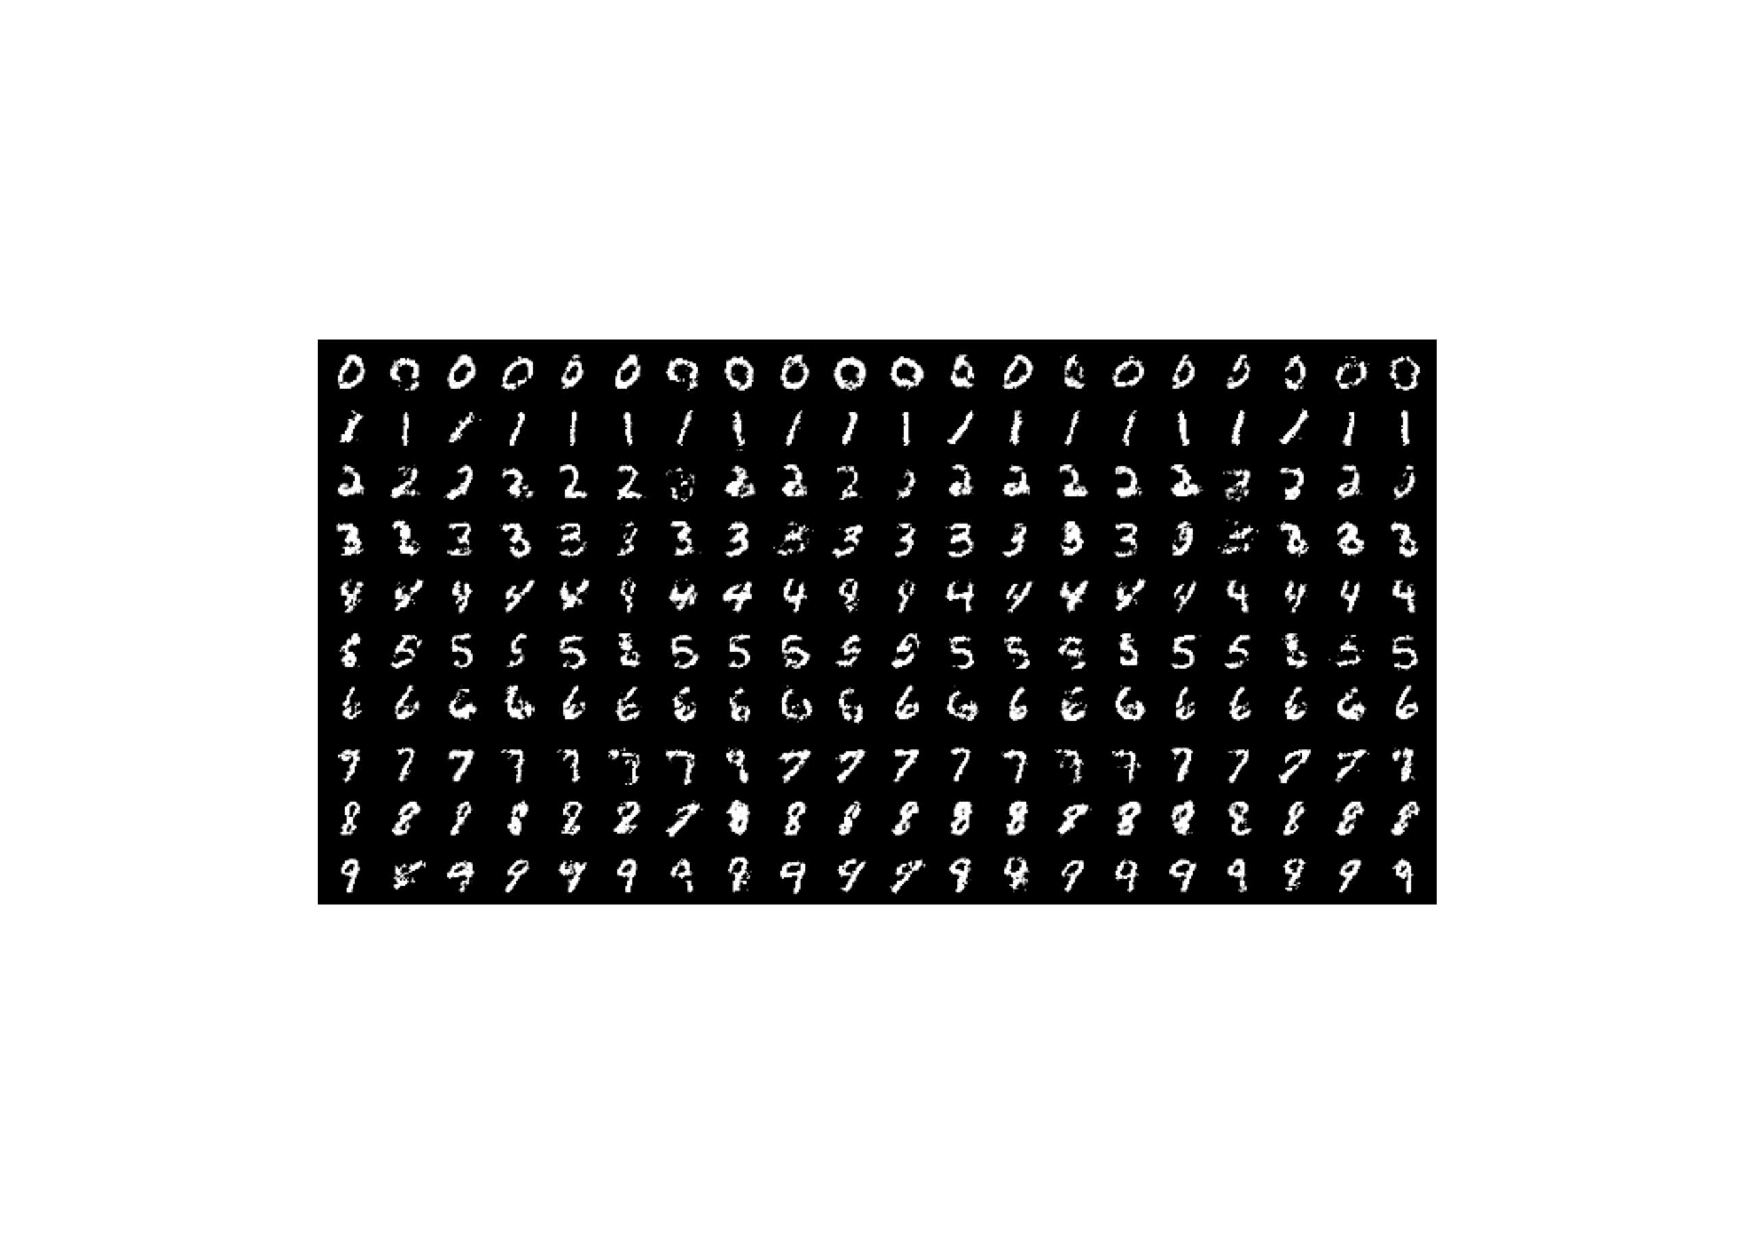
\includegraphics[width=\textwidth]{figures/CGAN-result.pdf}
    \caption{CGAN可以生成指定手写数字的类别。从上至下,CGAN生成了0-9总共10中类别的手写数字。}
    \label{CGAN-result}
\end{figure}

无论是GANs还是CGANs,此时仍受图像生成质量不高导致的实用价值不高的困扰。随着深度学习的发展,Alec Radford等人在2016年提出了使用卷积神经网络替换GANs中的多层感知机,大大提升了生成图像的质量。由于GANs已经广泛作为生成式对抗网络的概念使用,下文将称这Goodfellow等人提出的GANs模型为原始GANs。如图~\ref{GAN-DCGAN}所示,原始GANs生成的人像、自然图像质量都较差;而DCGAN能够生成较高质量的卧室图片。

\begin{figure}
    \centering
    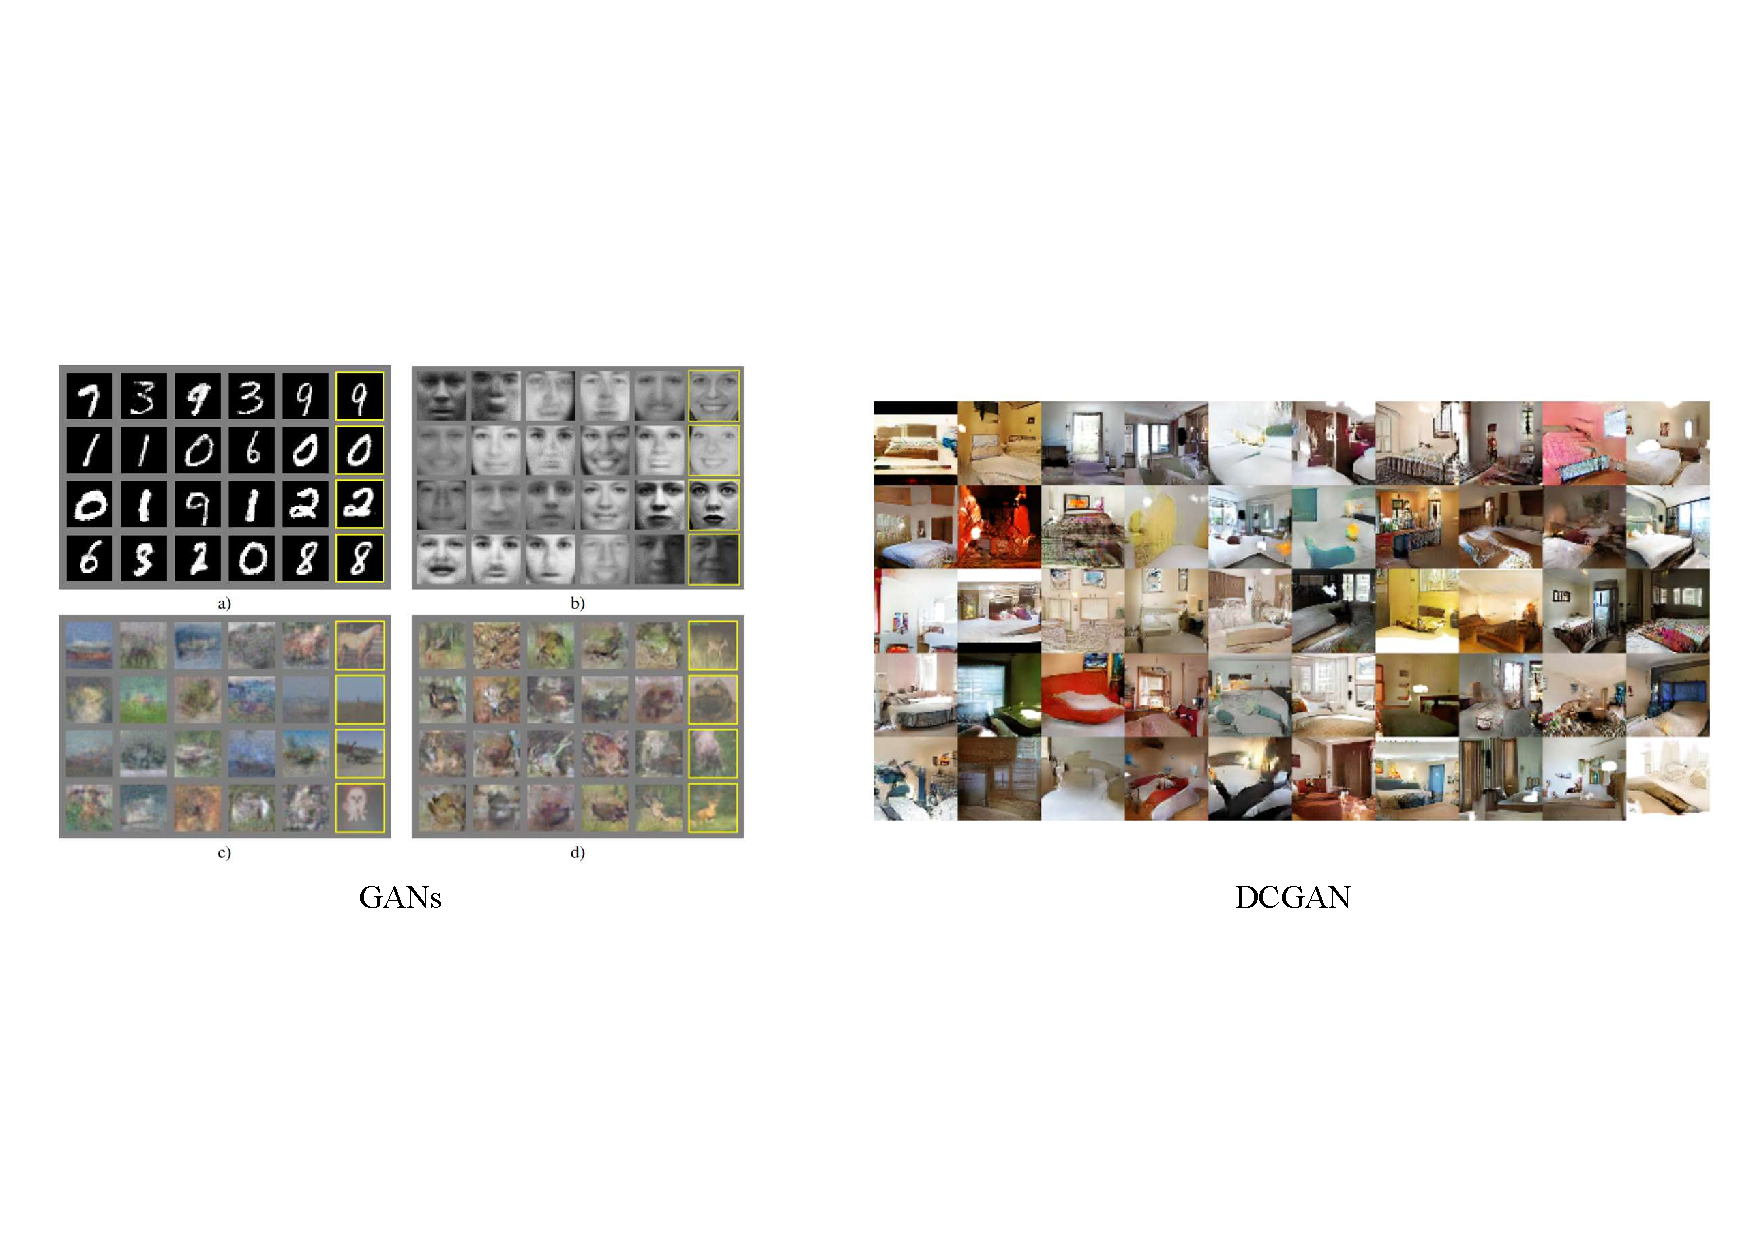
\includegraphics[width=\textwidth]{figures/GAN-DCGAN.pdf}
    \caption{GANs和DCGAN的生成效果对比}
    \label{GAN-DCGAN}
\end{figure}

至此,生成式对抗网络完成了它的萌芽阶段,其框架已经确定,最近的GANs模型基本都在这一框架内:

\begin{itemize}
\item GANs由生成器和判别器两个网络组成。
\item 训练采用对抗训练的方式。判别器致力于区分生成图像与真实图像,生成器目标是生成可以“骗过”判别器的图像。
\item 按照输入是否包含标签,GANs分为unconditional GANs和conditional GANs。
\item 就图像生成而言,生成器和判别器一般由卷积神经网络实现。
\end{itemize}

\subsection{发展:迈向以假乱真的真实图像和实际应用}
由于高分辨率图像包含更多细节,判别器更容易将生成的图像与真实图像区分开来,因此在高分辨率下训练GANs是一件很困难的事。除此之外,由于显存的限制,我们在高分辨率是只能使用较小的batch size,这进一步损害了训练时的稳定性。Odena等人在2017年提出PGGAN(Progressive Growing OF GANS)~\cite{PGGAN},作者认为可以从更简单的低分辨率图像开始逐步增加生成器和鉴别器,并随着训练的进行添加引入更高分辨率细节的新层。这种渐进式的训练方式大大加快了训练速度并提高了高分辨率下的稳定性。

时间来到2019年,BigGANs~\cite{BigGANs}探索了CGANs如何通过训练更大的模型提高生成图像的质量,StyleGAN~\cite{StyleGAN}则展示了GANs如何生成风格各异的图像。BigGANs和StyleGAN的生成结果分别如图~\ref{BigGAN}和图~\ref{StyleGAN}所示,可以看到无论是GANs(StyleGAN)还是CGANs(BigGANs),生成的图像都达到了“以假乱真”的程度。

\begin{figure}
    \centering
    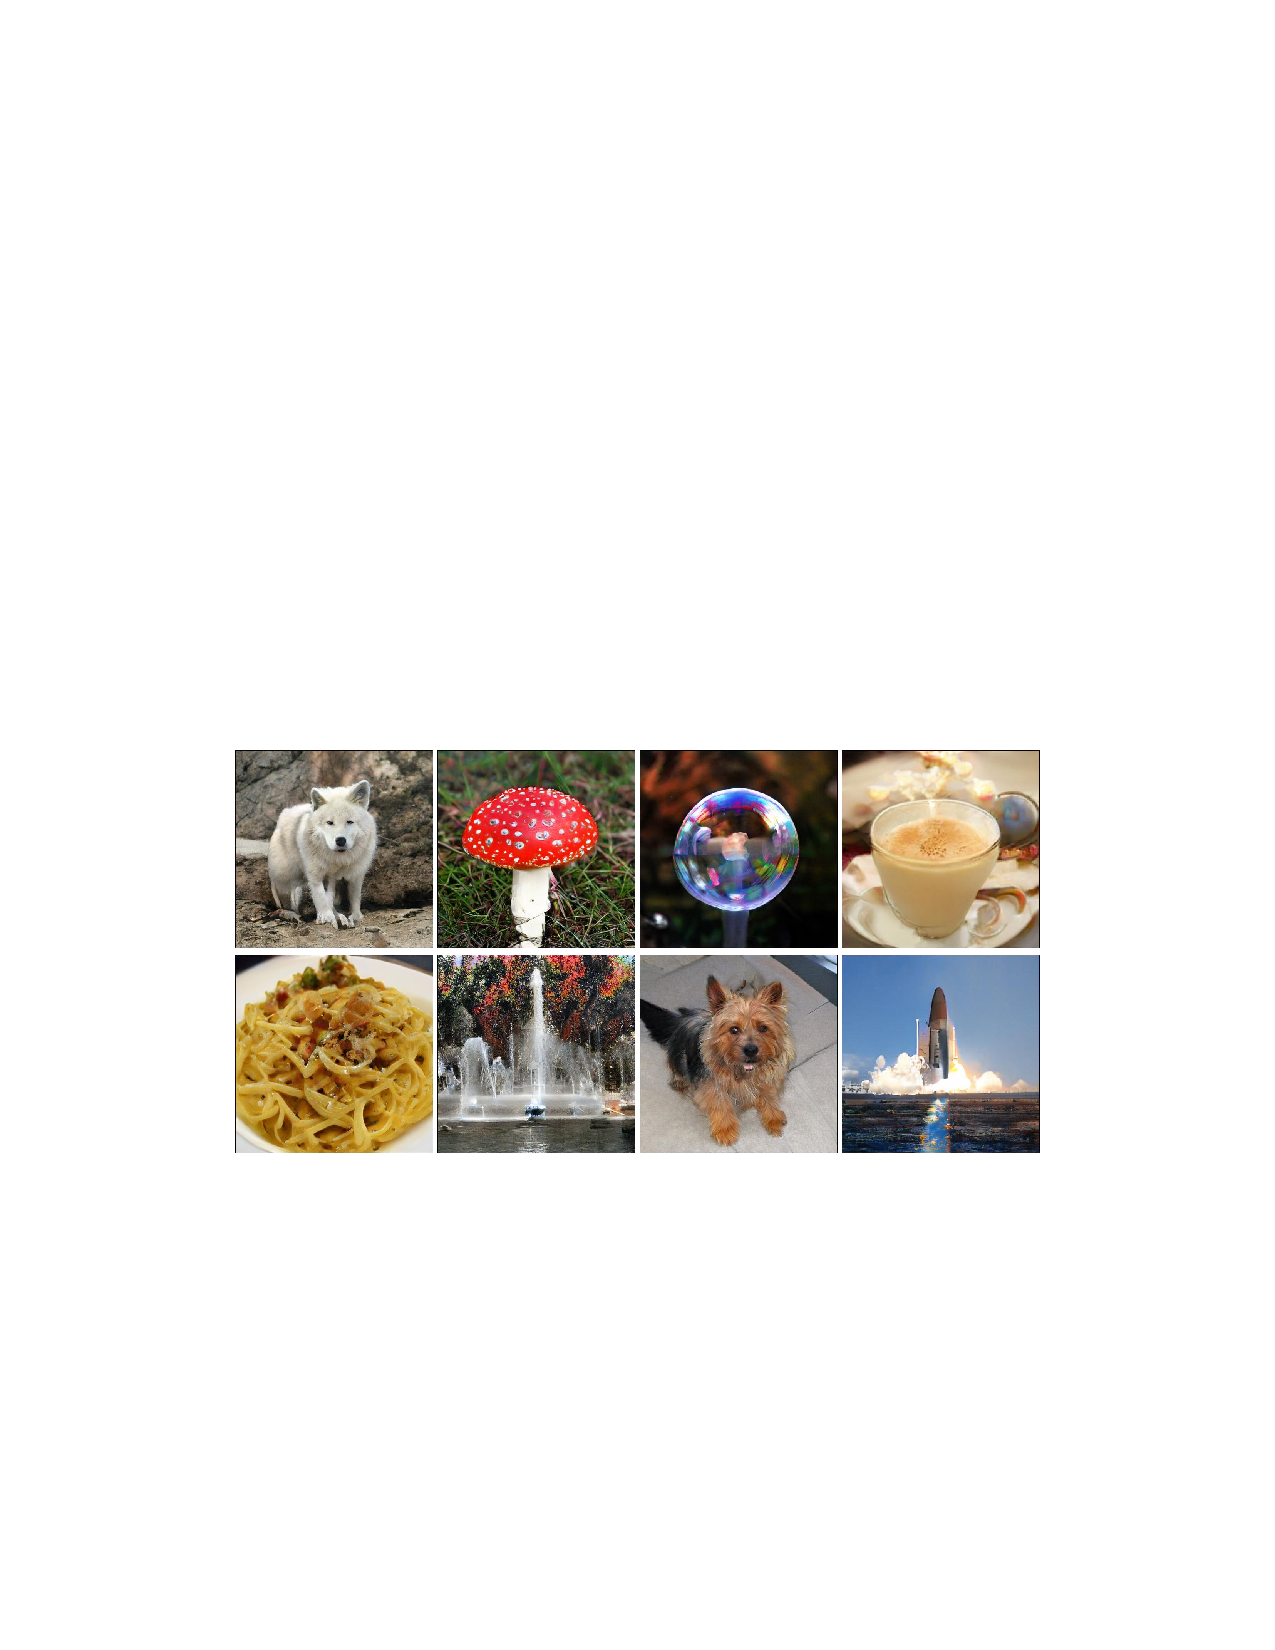
\includegraphics[width=\textwidth]{figures/BigGAN.pdf}
    \caption{BigGANs的512x512分辨率下的生成图像,可以看到生成的图像种类丰富且非常真实,但放大后仍可看出些许涂抹感。}
    \label{BigGAN}
\end{figure}

\begin{figure}
    \centering
    \includegraphics[width=\textwidth]{figures/StyleGAN.pdf}
    \caption{StyleGAN的生成结果。最上面一行与最左边一列是StyleGAN生成的不同风格的人像,中间则是两种风格混合后生成的人像。作者将这种风格混合生成人像的功能称为style mixing。}
    \label{StyleGAN}
\end{figure}


\subsection{最近进展和应用}

正如我们在上一节提到的,我们已经能够使用GANs生成足够真实且风格迥异的图片,因此研究热点逐渐转为GANs的应用。我们在这里主要介绍两类应用,一是基于GANs的属性编辑,二是基于GANs的图像转换。

CGANs的出现,使我们能够控制生成图像的类别,但我们仍无法控制生成图像的属性。例如,我们可以使用CGANs生成年轻人和老年人两类图像,但无法具体控制人物年轻或年老的程度。实际上早在DCGAN中,作者就发现了隐空间(生成器输入又称为隐变量,输入所在的空间又称为隐空间)中的向量运算可以控制生成图像的属性。受此启发,近些年出现了非常多通过在隐空间搜索语义方向的方式实现生成图像属性编辑的工作\cite{icml2020, harkonen2020ganspace, iclr2021, interfacegan, steer,variation},在这里我们将这类通过隐空间中向量预算改变生成图像属性的方法统称为隐空间编辑(latent-space editing)。

GANs很早就被用于图片转换(image translation),即将原域的图片转换为目标域的图片,经典的模型有Pix2Pix~\cite{pix2pix}、CycleGAN~\cite{cyclegan}等。本质上,这类用于图片转换的GANs是一种特殊的CGANs,此时原域的图片作为标签输入生成器。最近,研究人员提出CollaGAN~\cite{collagan}和Auto-GAN~\cite{AutoGAN},开始将GANs应用于多模态图像转换,一定程度上解决了多模态图像缺失的问题。


\section{问题和挑战}

据我们所知,现有的隐空间编辑均是:1.在预训练的GANs上搜索隐空间中属性对应的语义方向;2.在对应的语义方向上对隐变量进行向量运算。这类方法在做属性编辑时存在语义耦合的问题,即在改变某一属性时,其他属性也发生了变化。

在多模态图像变换方面,现有的基于GANs的方法没有充分利用模态间的一致性与互补性,这导致生成的目标模态图像出现信息损失。多模态数据广泛存在临床诊断等领域,缺失的信息可能会影响医生的决策。

\section{本文的贡献}

本文全面分析了GANs在属性编辑和多模态图像转换上遇到的问题和挑战,提供相应的解决方法:

(1)为了解决隐空间属性编辑语义耦合的问题,我们提出属性一致性网络。将输入隐变量分解为内容变量和属性变量,其中属性变量位于预定义的正交属性空间中,从而在理论上保证了属性编辑时的语义解耦。

(2)针对现有的基于GANs的多模态图像变换方法没有充分利用模态间的一致性与互补性的问题,我们提出联合注意力机制,在模型训练期间充分挖掘模态间的一致性与互补性,显著提高了多模态图像转换的质量与准确性。

\section{本文组织结构}

本文主要关注GANs在属性编辑和多模态图像转换上遇到的问题和挑战,提供相应的解决方案,并通过大量实验进行了验证,具体组织结构如下:

第一章简要梳理了生成对抗网络的发展历史,并引出了本文所关注的两个任务:属性编辑和多模态图像转换。最后总结了本文的创新点和贡献;

第二章全面介绍了生成对抗网络的原理与应用,特别是其在属性编辑和多模态图像上存在的不足;

第三章介绍了如何通过属性一致约束,实现天然能够控制属性连续变化的生成式对抗网络,从而解决隐空间属性编辑中的低效与耦合问题;

第四章介绍了如果使用注意力机制充分挖掘模态间的一致性与互补性,从而提高基于生成式对抗网络的多模态图像变换的质量;

第六章对全文进行总结,重点是本文的贡献和不足,为日后生成式对抗网络的研究提供了参考方向。
\clearpage{\pagestyle{empty}\cleardoublepage} % 去除空白页的页眉页脚(每章从奇数页开始,因此有空白页)
\chapter{相关概念及研究工作介绍}

\section{生成式对抗网络的理论}

\subsection{生成式对抗网络的概述}

基于生成式对抗网络~\cite{GANs}的生成模型极大的提升了图片生成的真实度。生成式对抗网络由生成器和判别器组成,生成器负责将隐变量(一般是从高斯分布采样的噪声)映射为生成的图像,判别器是一个二分类器,用于区分生成图像与真实图像。生成器和判别器以一种对抗的方式交替训练,这也是生成式对抗网络最核心的贡献。

受益于GANs广阔的应用前景,近来大量生成对抗网络相关的工作如雨后春笋般涌出,其中不乏一些重要的、对GANs理论和应用有深远影响的工作。原始GANs使用多层感知机(MLP)来实现,后来随着深度学习的发展,尤其是卷积神经网络在图像处理方面的广泛使用,Alec Radford等人在2016年提出了使用卷积神经网络替换GANs中的多层感知机~\cite{DCGAN},大大提升了生成图像的质量。在原始GANs中,生成器的输入是高斯噪声,这也就意味着你无法控制生成图像的类别。为了解决这个问题,Mehdi Mirza等人提出了条件生成式对抗网络(conditional GANs, cGANs)~\cite{CGANs},通过在输入中添加类别标签和在训练中添加分类损失,得到了能够指定生成数据类别的生成器。GANs自提出以来一直饱受训练不稳定问题的影响,Tim Salimans等人在Improved GANs~\cite{salimans2016improved}中总结了一系列训练技巧,目前已称为训练GANs的常规方案。还有一些文献~\cite{wgan, lsgan}则提出了新的损失函数,目的是更好地衡量生成数据与真实数据(训练集)分布的差距,从而提高GANs训练的稳定性。

目前GANs已经能够生成足够真实的图像,但仍需要很长的训练时间,以StyleGAN为例,在单Tesla V100显卡上训练需要接近70天!Bingchen Liu等人在2021年推出了一种轻量级GANs~\cite{lwgan},得益于其高效的网络结构和数据增广策略,只需要几个小时就能在单卡上完成训练。生成效果如图~\ref{fig:LWGAN}所示,可以看到这种轻量级GANs在生成质量上不如BigGANs、StyleGAN等重量级网络,但考虑到个人和科研机构往往计算资源有限,因此这类轻量级GANs仍有非常重要的现实意义。

\begin{figure}
    \centering
    \includegraphics[width=\textwidth]{figures/LWGAN.pdf}
    \caption{轻量级GANs在1024x1024分辨率下的生成效果}
    \label{fig:LWGAN}
\end{figure}

\subsection{损失函数}

我们用$\mathcal{L}_{GAN}(G, D)$表示GANs训练的损失函数。$\mathcal{L}_{GAN}(G, D)$的实现方式涉及到GANs训练的稳定性和生成数据的真实度,因此一直是GANs研究的重点问题。

在原始GANs中,$\mathcal{L}_{GAN}(G, D)$的计算如公式~\ref{eq:js_divergence}所示:

\begin{equation}
    \mathcal{L}_{GAN}(G, D) = E_{x \sim p_{\text {data }}(x)}[\log D(x)]+E_{z \sim p_{z}(z)}[\log (1-D(G(z)))]
    \label{eq:js_divergence}
\end{equation}

该公式本质上是生成数据与真实数据之间的JS散度。公式~\ref{eq:js_divergence}中的目标函数对训练生成器来说存在梯度消失的问题~\cite{review},解决这一问题一般的思路是重新设计目标函数。LSGAN~\cite{lsgan, lsgan2}提出使用最小二乘损失替代JS散度,WGAN~\cite{wgan}提出使用Wasserstein距离度量两个分布间的距离,Hinge损失的基本思想是让正例和负例之间的距离尽量大,最初用于支持向量机(SVM)的优化,后被迁移到GANs的训练~\cite{hinge1,hinge2,hinge3}。

\subsection{生成式对抗网络的训练}

生成器和判别器以一种对抗的方式交替训练,我们以先优化判别器为例,介绍GANs的训练流程。

在每次模型迭代中,我们先以公式~\ref{step_D}优化判别器,注意此时我们固定生成器的权重不变。

\begin{equation}
    \max _{D} V(D, G, R) = \mathcal{L}_{GAN}(G, D)
    \label{step_D}
\end{equation}

然后,我们以公式~\ref{step_G}优化生成器,同样的,此时我们固定判别器的权重不变。

\begin{equation}
    \min _{G} V(D, G, R) = \mathcal{L}_{GAN}(G, D)
    \label{step_G}
\end{equation}

将公式~\ref{step_D}和~\ref{step_G}结合起来,我们就得到了如公式~\ref{overall}所示的GANs总损失。

\begin{equation}
    \min _{G} \max _{D} V(D, G, R) = \mathcal{L}_{GAN}(G, D)
\end{equation}

重复上述步骤,直到生成器生成的图像对人来说足够真实,生成图像的真实度也可以用FID~\cite{fid}等评价指标辅助判断。与其他机器学习模型不同,生成器和判别器的损失并不能直接表明模型的好坏,需要我们通过观察生成图像的质量来判断训练进度。

\subsection{生成图像的评价指标}

我们在这里重点介绍4种生成图像的评价指标,分别是SSIM、FSIM、IS和FID,这些评价指标从不同的角度评估了生成图像的真实性,需要根据具体的任务来选择何时的评价指标。

SSIM(Structural Similarity Index Measure,结构相似性)~\cite{ssim},是一种衡量两张图片结构相似性的指标,最初用于比较无失真图像和压缩后失真影像的相似性,可看作失真影像质量的评价指标,现也用于比较任意两张图像的结构相似性。计算公式如下所示:

\begin{equation}
    \operatorname{SSIM}(x, y)=\frac{\left(2 \mu_{x} \mu_{y}+c_{1}\right)\left(2 \sigma_{x y}+c_{2}\right)}{\left(\mu_{x}^{2}+\mu_{y}^{2}+c_{1}\right)\left(\sigma_{x}^{2}+\sigma_{y}^{2}+c_{2}\right)}
\end{equation}
在这里$x$,$y$表示用于比较的两张图片,$\mu_{x}$是$x$的平均值,$\mu_{y}$为$y$的平均值,$\sigma_{x}^{2}$为的$x$方差,$\sigma_{y}^{2}$为$y$的方差,$\sigma_{x y}$为$x$,$y$的协方差。$c_{1}$与$c_{2}$均为常数,用来维持数值稳定。

FSIM(Feature Similarity Index Measure,特征相似性)~\cite{fsim},概念与SSIM类似,考察两张图像特征的相似性。

IS(Inception Score)~\cite{salimans2016improved}对每张生成图像,使用Inception模型~\cite{inception}计算条件标签分布$p(y|x)$。如果生成图像中包含有意义的物体,那么计算条件标签分布$p(y|x)$的值应该较低。另一方面,我们希望生成图像尽可能多样化,反映在边缘概率$\int p(y \mid x=G(z)) dz$上应该是较大的值。结合上述两点,IS的计算公式为:

\begin{equation}
    IS\left(p(y \mid x), p(y)\right)=\exp \left(E_{x} K L(p(y \mid x) \| p(y))\right)
\end{equation}

更高的IS分数意味着生成器能够生成具有明确语义且多样化的图像。然而,IS分数也有其劣势,如果生成模型陷入模式坍塌,IS分数可能仍然较低。

FID(Fréchet Inception Distance)~\cite{fid}是专为GANs设计的评价指标,计算方式是使用Inception模型的卷积层特征计算函数$\phi$,对真实数据分布$p_{data}$和生成数据分布$p_{g}$建模为高斯随机变量$\phi (p_{data})$和$\phi (p_{g})$,其均值为$\mu_{r}$, $\mu_{g}$,方差为$C_{r}$, $C_{g}$,最后计算:
\begin{equation}
    F I D\left(p_{\text {data }}, p_{g}\right)=\left\|\mu_{r}-\mu_{g}\right\| + tr\left(C_{r}+C_{g}-2\left(C_{r} C_{g}\right)^{1 / 2}\right)
\end{equation}
即可得到FID分数,本质上是这两个高斯分布之间的弗雷歇距离(Fréchet distance)。

\section{生成式对抗网络的应用}

\subsection{图像转换}

图像转换(Image translation)指将输入图像从原风格转换为目标风格(风格转换)或从原图像域转换为目标图像域。 随着深度学习的发展,神经网络风格迁移(neural sytle transfer)~\cite{transfer0,transfer1,transfer2}已经成为风格迁移的主流方法。 风格迁移侧重于不同的艺术风格间的转换,而图像转换~\cite{i2i0,i2i1,i2i2,cyclegan} 解决了更一般的图像域转换问题。

不同的图像转换方法侧重于从不同的角度,解决不同类型的图像转换问题。Pix2Pix~\cite{pix2pix}解决了配对图像(像素对齐的两张图像)的图像转换问题。对于损失函数,Pix2Pix的作者认为可以依靠L1损失约束低频信息,判别器仅用来鉴别高频信息是否真实,作者进一步提出了PatchGAN。 PatchGAN的核心思想是,既然判别器只用于鉴别高频信息,那么就不需要将整张图片输入到判别器中,只在patch(正方形像素块,作者最终采用了70x70的像素块作为patch)的规模上计算高频结构损失。因为不同的patch之间可以认为是相互独立的。PatchGAN对一张图片切割成不同的N x N大小的patch,判别器对每一个patch做真假判别,将一张图片所有patch的结果取平均作为最终的判别器输出。作者认为这会鼓励GANs生成的图像包含清晰的高频细节。

现实世界中更一般的实际上是非配对图像的转换,因为配对图像在大部分真实场景非常难以获取,比如我们要做马和斑马之间的转换,几乎不可能找到像素点对齐的马和斑马的配对图像。
CycleGAN~\cite{cyclegan}提出了循环一致性损失解决了非配对图像的转换问题。与常规的GANs不同,CycleGAN包含两个生成器$G_A$和$G_B$,与两个判别器$D_A$和$D_B$。假设我们有两张分别来自于$A$图像域和$B$图像域的图片$I^A$和$I^B$,非配对图像转换的难点在于,如果我们要将$I^A$转换到$B$域,我们没有$I^A$在$B$域的对应图像,因此无法用类似L1损失的方式约束像素之间的差异。在计算循环一致性损失时,先用$G_A$将$I^A$转换到$B$域,再用$G_B$将上一步的结果转换回$A$域,得到$I^A_{cyc}$,此时就可以计算$I^A$和$I^A_{cyc}$之间的差异,$I^B$和$I^B_{cyc}$的计算类似,如公式~\ref{eq:cyc}所示。

\begin{equation}
    \mathcal{L}_{\mathrm{cyc}}(G, F) =\mathbb{E}_{x \sim p_{\text {data }}(x)}\left[\|F(G(x))-x\|_{1}\right] +\mathbb{E}_{y \sim p_{\text {data }}(y)}\left[\|G(F(y))-y\|_{1}\right]
    \label{eq:cyc}
\end{equation}

无论是Pix2Pix还是CycleGAN,都是解决了两个图像域之间的转换,如果需要多个域之间互相转换,只能训练多个模型,StarGAN~\cite{stargan}通过在输入增加目标域对应的掩码(mask)和类别损失,使用单一模型解决了多个域之间互相转换的问题。

图像转换方法从整体来看,都是输入一张图像,然后转换为另一张图像,与下面要介绍的隐空间编辑方法有很大不同,因此一部分文献~\cite{iclr2021}将图像转换又称为图像空间编辑。目前大多数基于GANs的图像空间编辑方法的问题在于难以同时编辑多个属性,并精确控制生成图像中的属性强度。

\subsection{隐空间编辑}

在GANs发展的早期,Alec Radford等人就在\cite{DCGAN}中发现GANs的隐空间中通常包含有语义意义的向量算法,例如,隐空间中存在能为人脸添加微笑或眼镜的方向。我们称这类通过隐空间向量运算实现图像编辑发方法为隐空间编辑方法,区别与上文提到的图像空间编辑方法,后者是对图像直接的转换。

由于隐空间编辑使图像编辑更加简单,因此近些年来这类方法收到越来越到的关注。从隐空间编辑的监督方式来看,隐空间编辑方法分为有监督、无监督、自监督或半监督的方法。

\begin{enumerate}
\item 有监督的隐空间编辑方法采用明确的人工监督来识别隐空间中的可解释方向,如Yujun Shen等人~\cite{interfacegan}使用在CelebA数据集~\cite{celeba}上预训练的二分类器来预测人脸属性。然后使用该分类器为生成的图像及对应的隐变量生成伪标签。基于这些伪标签,可以在隐空间空间中构建分类超平面,该超平面的法线即为相应属性变化的方向。

\item 无监督通过学习一组语义上区别较大的方向~\cite{icml2020} 或基于主成分分析(PCA)的方法~\cite{harkonen2020ganspace}识别潜在的的语义方向。这些方法可能会找到有意义的方向,但其结果是不可预测的,并且需要人工解释,这导致了非监督的隐空间编辑方法难以指定所需的语义方向。

\item 自监督方法~\cite{steer,variation} 通过使用简单的几何变换(例如旋转和缩放)增加数据来搜索可解释的方向,这限制了这些方法搜索复杂属性的能力。半监督方法~\cite{nie2020semi} 调查了有限监督的影响,这很难同时精准解耦并编辑多个属性。
\end{enumerate}

以上方法的本质均是在预训练的GANs的隐空间中搜索语义方向,不可避免地受到预训练GANs的影响,由于GANs在训练时没有受到语义属性的约束,其隐空间必然存在语义耦合现象。这导致现有的隐空间编辑的方法在改变某一属性时,通常会导致其他的属性也发生变化。    

\subsection{多模态图像转换}

在图像处理、计算机视觉和计算机图形学的许多应用中,越来越依赖于多模态医学图像。例如精准医学,脑部核磁共振中存在T1、T1Gd、T2和T2-FLAIR四种模态~\cite{drevelegas2011imaging}。医生希望结合完整的多模态医学图像来做出更精确的诊断,但受限于实际条件限制(例如,受限的医疗条件、扫描时间不足以及成本/支出/资源等限制),实践中可能存在成像系统存在误差,甚至部分模态的缺失的现象~\cite{tanenbaum2017synthetic}。这些不可用的图像可能会导致医生决策出现偏差。

Dongwook Lee等人提出的CollaGAN~\cite{collagan}是第一篇将GANs用于多模态图像。与CycleGAN,Pix2Pix等单模态图像转换方法只能输入一种模态的图像不同,CollaGAN针对多模态图像转换提出了多重循环一致损失(Multiple cycle consistency loss),通过一个GANs模型解决了多模态间模态转换的问题。

CollaGAN和Auto-GAN均使用单个模型在一定程度上解决了多模态图像转换的问题,但都没有在训练过程中对模态间的一致性和互补性进行约束。

\section{本章小结}

在本章节我们总结了生成式对抗网络,图片空间编辑、隐空间编辑和多模态图像转换的原理、应用和进展,重点梳理了隐空间编辑和多模态图像现有方法的优势与不足,为后续本文解决方案的提出奠定了基础。

\clearpage{\pagestyle{empty}\cleardoublepage}
\chapter{总结与展望}

\section{全文总结}

生成式对抗网络(GANs)自提出以来就一直是深度学习乃至人工智能领域的热门话题。在近几年研究人员的持续努力之下,GANs在训练稳定性、生成图像的质量方面取得了长足的进步。随着GANs生成图像真实度越来越接近真实图像,研究人员开始探索GANs的具体应用。本文梳理了GANs的发展历程和应用领域,就图像编辑和多模态图像转换展开了讨论,指出目前所存在的问题,并给出了相应的解决方案。

为了隐空间编辑语义耦合的问题,并更准确地控制生成图像的属性,本文提出了属性一致生成对抗网络(Attribute Consistent Generative Adversarial Networks),简称ACGAN。为了证明ACGAN可基于任意非条件GANs实现,本文在StyleGAN2和文献~\cite{lwgan}提出的轻量级GANs的基础上实现了ACGAN,分别用于人脸属性编辑和自然风景属性编辑。为了全面分析与展示ACGAN在属性编辑方面的优越性,本文对这两种场景下的属性编辑均设计了对应的定量与定性两类实验,其中不乏人脸属性编辑中的属性编辑成功率与保留率,和自然风景属性编辑中属性增益这样原创性的评价指标。为了将ACGAN拓展到现有的二值属性标注数据集,本文还提出了一种属性量化策略,用于生成连续的伪标签。

为了解决难以对多模态输入之间相关性建模的问题,本文提出了一种联合注意力生成式对抗网络 (Joint Attetion Generative Adversarial Networks, JAGAN),探索了如何通过注意力机制通过挖掘模态间的一致性与互补性,提出了模态内注意力和模态间注意力两种注意力机制,高效实现了利用多模态图像补全缺失的模态图像。本文在医学图像转换和面部图像转换两个场景下做了实验,展示了JAGAN相对于现有图像转换方法在多模态场景下的优越性。然后,本文通过消融实验证明了两种注意力机制的有效性,和两种注意力结合使用的必要性。

本文的贡献可归纳为以下几点:

(1)第三章提出了属性一致生成对抗网络ACGAN:GAN的隐空间被分解为内容空间和正交的语义空间,为解决隐空间编辑语义耦合问题提供了理论上的保障。本文提出属性一致性损失,引入属性回归器在训练阶段监督输入属性与生成图像属性之间的一致性。ACGAN统一了GANs生成图像与属性控制两个任务,使生成器天然具有控制生成图像属性的能力。

(2)在第三章中,为了将ACGAN应用于更常见的二值属性数据集,本文设计了一种属性量化方法,来获得连续属性伪标签。这种属性量化方法可以灵活地与现有方法集成以提高属性编辑性能。

(3)第四章提出了联合注意力生成式对抗网络JAGAN。针对多模态图像转换,提出跨模态一致性和模态间互补性的概念,指出现有方法的不足。模态内注意力依据跨模态一致性,借助自表示网络来引导生成器的训练,在特征提取阶段过滤掉无关信息,并模态信息互补提供了所需的特征兼容。模态间注意力依据模态间互补性,为每个输入模态补充生成目标模态所需要的信息。

\section{展望}

虽然我们在第三章提出的 ACGAN 与现有的隐空间编辑和图像转换方法相比实现了更加卓越的性能,但仍存在一些局限性。例如,在计算属性一致性损失时,从均匀分布采样可能会采样到矛盾的属性组合,使用图卷积神经网络(GCN)辅助采样将是非常值得尝试的方案。 此外,对真实图像的编辑十分依赖GAN逆映射(GAN inversion)的效果,这通常需要复杂的 GAN 架构,如StyleGAN2 。然而,使用StyleGAN2 实现ACGAN需要大量的训练时间。第四章提出的 JAGAN 同样存在类似的问题:JAGAN与其他最先进的技术相比实现了卓越的性能,但需要更多的计算资源和计算时间。未来,我们将探索更高效的GAN架构。

除了本文所提到的GANs在图像编辑和多模态图像转换方面的应用外,GANs实际上还有许多方面的应用,如国际计算机视觉大会(ICCV)2019最佳论文SinGAN~\cite{singan}使用单一GANs模型实现了图像相关的5种任务。除图像外,GANs还可用于语音、音乐的合成~\cite{voice1,voice2,voice3}。GANs在特定领域的应用方兴未艾,存在大量问题需要解决,值得所有GANs研究人员继续努力。
\clearpage{\pagestyle{empty}\cleardoublepage}
%%%%%%%%%% 正文部分内容  %%%%%%%%%%

%%%%%%%%%%  参考文献  %%%%%%%%%%
\defaultfont
\bibliographystyle{references/TJUThesis}
\phantomsection
\markboth{参考文献}{参考文献}
\addcontentsline{toc}{chapter}{参考文献}          % 参考文献加入到中文目录
% \nocite{*}                                       % 若将此命令屏蔽掉,则未引用的文献不会出现在文后的参考文献中。
\bibliography{references/reference}

\clearpage{\pagestyle{empty}\cleardoublepage}
% !Mode:: "TeX:UTF-8"

\markboth{发表论文和参加科研情况说明}{发表论文和参加科研情况说明}
\addcontentsline{toc}{chapter}{发表论文和参加科研情况说明}
\chapter*{发表论文和参加科研情况说明}
\setlength{\parindent}{0em}
% \textbf{(一)发表的学术论文}
% \begin{publist}
% \item XXX,XXX. Density and Non-Grid based Subspace Clustering via Kernel Density Estimation[C]. ECML-PKDD 2012, Bristol, UK.(Submitted, Under review)
% \item XXX,XXX. A tree parent storage based on hashtable for XML construction[C]. Communication Systems, Networks and Applications, Hongkong, 2010: 325-328. (EI DOI: 10.1109/ICCSNA.2010.5588732)
% \end{publist}

\vspace*{1em}
\textbf{(一)申请及已获得的专利(无专利时此项不必列出)}
\begin{publist}
\item [1]朱鹏飞, 刘家旭, 汪廉杰,等. 一种人机协同的图像目标检测数据半自动标注方法。
\end{publist}
\vspace*{1em}
% \textbf{(三)参与的科研项目}
% \begin{publist}
% \item	XXX,XXX. XX~信息管理与信息系统, ~国家自然科学基金项目.课题编号:XXXX.
% \end{publist}
\vfill
\hangafter=1\hangindent=2em\noindent

\setlength{\parindent}{2em}                   % 发表论文和参加科研情况说明
\clearpage{\pagestyle{empty}\cleardoublepage}
\markboth{致\quad 谢}{致\quad 谢}
\addcontentsline{toc}{chapter}{致\qquad 谢} %添加到目录中
\chapter*{致\qquad 谢}

在这里,我首先要感谢导师朱鹏飞副教授。朱老师是我科研道路上的引路人,在如何阅读文献、如何寻找科研灵感、如何设计实验等十分重要的科研技能方面给予了我全方位的指导。朱老师本人博学的知识,对科研事业的坚持,深深的感染了我,使我对科研产生既有严谨的态度,又有充足的热情。朱老师培养了我扎实的科研基础与严谨的科研习惯,并为了我规划了科研的方向。

然后我要感谢曹兵老师。成功的科研工作背后有无数细节上的困难,曹老师去年刚刚博士毕业,每当遇到细节上的困时,活跃在科研一线的曹老师都会与我讨论,帮我分析问题,并得出切实可行的方案。当我实验失败,情绪低落时,曹老师会以讲他本硕期间的经历、带我打羽毛球放松等方式鼓励我。总之,感谢曹兵老师这几个月以来的授业解惑。

最后我要感谢家人和同学,正是有了你们的鼓励与支持,我才能无惧困难,以积极的态度、饱满的的热情完成本文中的两个工作。我相信致谢不是别离,我希望在今后的日子里,能与各位老师、同学保持紧密的联系,共创更加美好的未来!
               % 致谢
\clearpage
\end{document}                                 % 结束全文
